\section{Seq2Seq Architecture}
\begin{frame}{}
  \LARGE \textbf{Seq2Seq Architecture}
\end{frame}

\begin{frame}{Seq2Seq Architecture}
  \textbf{Key Idea:} Map input sequence $\rightarrow$ intermediate vector $\rightarrow$ output sequence.
  \vspace{1em}
  \begin{itemize}
    \item[\textcolor{red}{$\blacktriangleright$}] \textbf{Encoder RNN:} Processes input sequence and compresses it into a \textbf{fixed-length vector} (context).
    \item[\textcolor{red}{$\blacktriangleright$}] \textbf{Decoder RNN:} Generates output sequence from the context vector.
  \end{itemize}
  \vspace{1em}
  \textbf{Applications:}
  \begin{itemize}
    \item[\textcolor{red}{$\blacktriangleright$}] Machine translation
    \item[\textcolor{red}{$\blacktriangleright$}] Summarization
    \item[\textcolor{red}{$\blacktriangleright$}] Dialogue systems
    \item[\textcolor{red}{$\blacktriangleright$}] Speech recognition
  \end{itemize}
\end{frame}

% Slide 8
\begin{frame}{Seq2Seq Architecture}
  \centering
  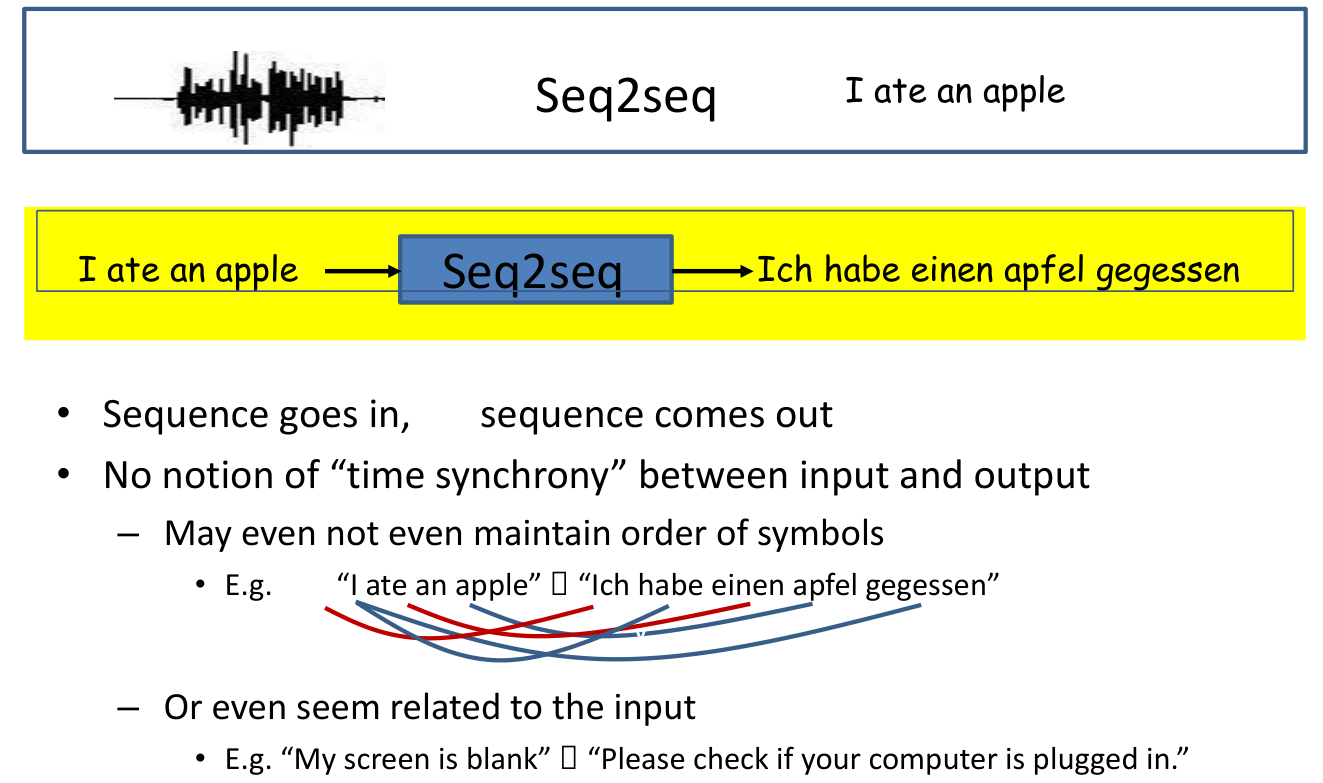
\includegraphics[width=0.35\paperwidth,height=0.35\paperheight,keepaspectratio]{assets/Lecture-4_Sequence_to_Sequence_Models_Intro_to_Attention/slide_008.png}
\end{frame}

\begin{frame}{Modeling the problem}
  \centering
  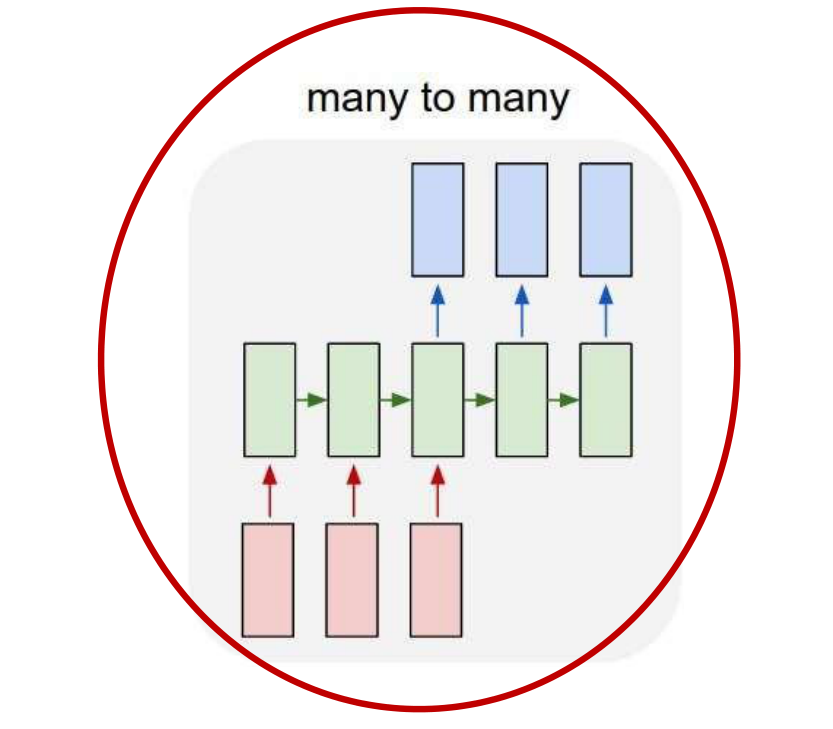
\includegraphics[width=0.35\paperwidth,height=0.35\paperheight,keepaspectratio]{assets/Lecture-4_Sequence_to_Sequence_Models_Intro_to_Attention/slide_009.png}
  \centering
  \textit{Delayed} sequence to sequence
\end{frame}

\begin{frame}{Modeling the problem}
  \centering
  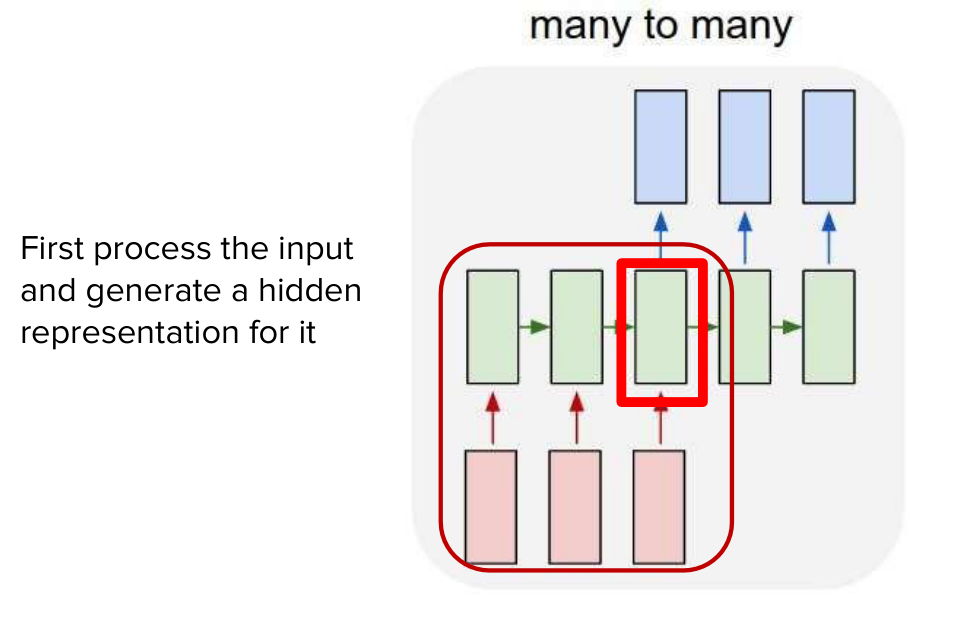
\includegraphics[width=0.35\paperwidth,height=0.35\paperheight,keepaspectratio]{assets/Lecture-4_Sequence_to_Sequence_Models_Intro_to_Attention/slide_010.png}
  \centering
  \LARGE \textit{Delayed} sequence to sequence
\end{frame}

% Slide 11
\begin{frame}{Modeling the problem}
  \centering
  
\includegraphics[width=0.35\paperwidth,height=0.35\paperheight,keepaspectratio]{assets/Lecture-4_Sequence_to_Sequence_Models_Intro_to_Attention/slide_011.png}
  \LARGE \textit{Delayed} sequence to sequence
\end{frame}

% Slide 12
\begin{frame}{Modeling the problem}
  \centering
  
\includegraphics[width=0.35\paperwidth,height=0.35\paperheight,keepaspectratio]{assets/Lecture-4_Sequence_to_Sequence_Models_Intro_to_Attention/slide_012.png}
  \textit{Problem:} Each word that is output depends only on  current hidden state, and not on previous outputs
\end{frame}

% Slide 13
\begin{frame}{Modeling the problem}
  \centering
  
\includegraphics[width=0.35\paperwidth,height=0.35\paperheight,keepaspectratio]{assets/Lecture-4_Sequence_to_Sequence_Models_Intro_to_Attention/slide_013.png}
  \centering
  \begin{itemize}
    \item \textit{Delayed} Sequence to sequence
    \begin{itemize}
    \item Delayed \textit{self-referencing} sequence-to-sequence
    \end{itemize}
  \end{itemize}
\end{frame}

% Slide 14
\begin{frame}{The “simple” translation model}
  \centering
  
\includegraphics[width=0.35\paperwidth,height=0.35\paperheight,keepaspectratio]{assets/Lecture-4_Sequence_to_Sequence_Models_Intro_to_Attention/slide_014.png}
  \begin{itemize}
    \item The input sequence feeds into a recurrent structure 
    \item The input sequence is terminated by an explicit \texttt{<eos>} symbol 
    \begin{itemize}
        \item \textcolor{red}{The hidden activation at the \texttt{<eos>} ``stores'' all information about the sentence} 
    \end{itemize}
\end{itemize}  
\end{frame}

% Slide 15
\begin{frame}{The “simple” translation model}
  \centering
  
\includegraphics[width=0.35\paperwidth,height=0.35\paperheight,keepaspectratio]{assets/Lecture-4_Sequence_to_Sequence_Models_Intro_to_Attention/slide_015.png}
  \begin{itemize}
    \item The input sequence feeds into a recurrent structure 
    \item The input sequence is terminated by an explicit \texttt{<eos>} symbol 
    \begin{itemize}
        \item The hidden activation at the \texttt{<eos>} ``stores'' all information about the sentence 
    \end{itemize}
    \item Subsequently a second RNN uses the hidden activation as initial state, and \texttt{<sos>} as initial symbol, to produce a sequence of outputs
    \begin{itemize}
        \item The output at each time becomes the input at the next time 
        \item Output production continues until an \texttt{<eos>} is produced 
    \end{itemize}
\end{itemize}  
\end{frame}

% Slide 16
\begin{frame}{The “simple” translation model}
  \centering
  
\includegraphics[width=0.35\paperwidth,height=0.35\paperheight,keepaspectratio]{assets/Lecture-4_Sequence_to_Sequence_Models_Intro_to_Attention/slide_016.png}
  \begin{itemize}
    \item The input sequence feeds into a recurrent structure
    \item The input sequence is terminated by an explicit \texttt{<eos>} symbol
    \begin{itemize}
        \item The hidden activation at the \texttt{<eos>} ``stores'' all information about the sentence
    \end{itemize}
    \item Subsequently a second RNN uses the hidden activation as initial state to produce a sequence of outputs
    \begin{itemize}
        \item The output at each time becomes the input at the next time
        \item Output production continues until an \texttt{<eos>} is produced
    \end{itemize}
\end{itemize}  
\end{frame}

% Slide 17
\begin{frame}{The “simple” translation model}
  \centering
  
\includegraphics[width=0.35\paperwidth,height=0.35\paperheight,keepaspectratio]{assets/Lecture-4_Sequence_to_Sequence_Models_Intro_to_Attention/slide_017.png}
  \begin{itemize}
    \item The input sequence feeds into a recurrent structure
    \item The input sequence is terminated by an explicit \texttt{<eos>} symbol
    \begin{itemize}
        \item The hidden activation at the \texttt{<eos>} ``stores'' all information about the sentence
    \end{itemize}
    \item Subsequently a second RNN uses the hidden activation as initial state to produce a sequence of outputs
    \begin{itemize}
        \item The output at each time becomes the input at the next time
        \item Output production continues until an \texttt{<eos>} is produced
    \end{itemize}
\end{itemize}  
\end{frame}

% Slide 18
\begin{frame}{The “simple” translation model}
  \centering
  
\includegraphics[width=0.35\paperwidth,height=0.35\paperheight,keepaspectratio]{assets/Lecture-4_Sequence_to_Sequence_Models_Intro_to_Attention/slide_018.png}
  \begin{itemize}
    \item The input sequence feeds into a recurrent structure 
    \item The input sequence is terminated by an explicit \texttt{<eos>} symbol 
    \begin{itemize}
        \item The hidden activation at the \texttt{<eos>} ``stores'' all information about the sentence 
    \end{itemize}
    \item Subsequently a second RNN uses the hidden activation as initial state to produce a sequence of outputs 
    \begin{itemize}
        \item The output at each time becomes the input at the next time 
        \item Output production continues until an \texttt{<eos>} is produced 
    \end{itemize}
\end{itemize}
\end{frame}

% Slide 19
\begin{frame}{The “simple” translation model}
  \centering
  
\includegraphics[width=0.35\paperwidth,height=0.35\paperheight,keepaspectratio]{assets/Lecture-4_Sequence_to_Sequence_Models_Intro_to_Attention/slide_019.png}
  \begin{itemize}
    \item The input sequence feeds into a recurrent structure 
    \item The input sequence is terminated by an explicit \texttt{<eos>} symbol 
    \begin{itemize}
        \item The hidden activation at the \texttt{<eos>} ``stores'' all information about the sentence 
    \end{itemize}
    \item Subsequently a second RNN uses the hidden activation as initial state to produce a sequence of outputs 
    \begin{itemize}
        \item The output at each time becomes the input at the next time 
        \item Output production continues until an \texttt{<eos>} is produced 
    \end{itemize}
\end{itemize}
\end{frame}

% Slide 20
\begin{frame}{The “simple” translation model}
  \centering
  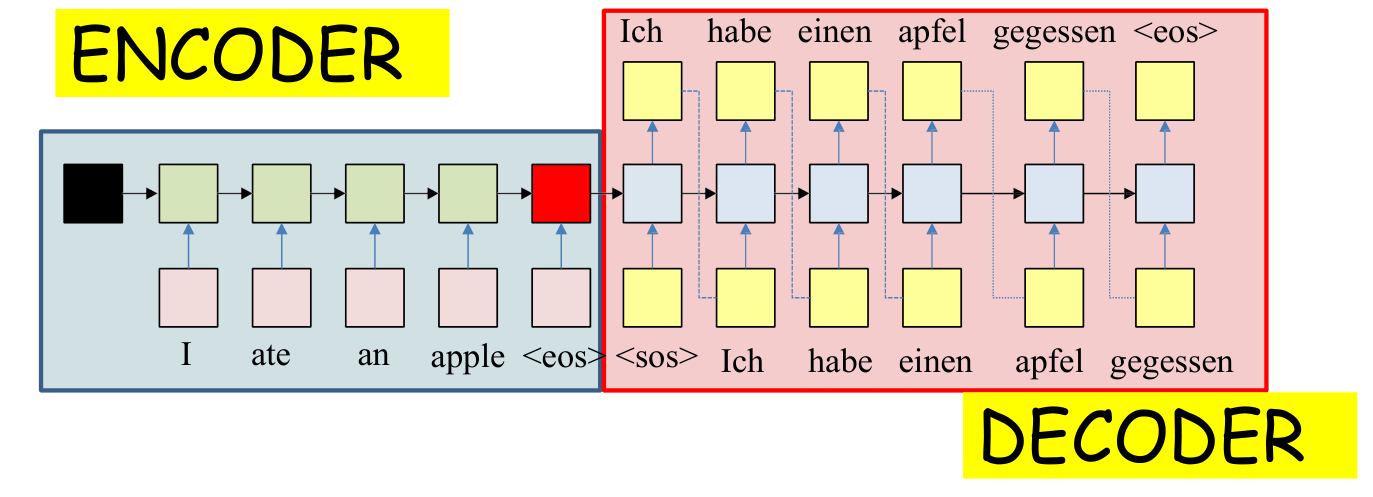
\includegraphics[width=0.35\paperwidth,height=0.35\paperheight,keepaspectratio]{assets/Lecture-4_Sequence_to_Sequence_Models_Intro_to_Attention/slide_020.png}
  \begin{itemize}
    \item The recurrent structure that extracts the hidden representation from the input sequence is the \textbf{encoder} 
    \item The recurrent structure that utilizes this representation to produce the output sequence is the \textbf{decoder}
  \end{itemize}  
\end{frame}